%%%%%%%%%%%%%%%%%%%%%%%%%%%%%%%%%%%%%%%%%%%%%%%%%%%%%%%%%%%%%%%%%%%%%%
% LaTeX Example: Project Report
%
% Source: http://www.howtotex.com
%
% Feel free to distribute this example, but please keep the referral
% to howtotex.com
% Date: March 2011 
% 
%%%%%%%%%%%%%%%%%%%%%%%%%%%%%%%%%%%%%%%%%%%%%%%%%%%%%%%%%%%%%%%%%%%%%%

% Edit the title below to update the display in My Documents
%\title{Project Report}
%
%%% Preamble
\documentclass[paper=a4, fontsize=11pt]{scrartcl}
\usepackage[T1]{fontenc}
\usepackage{fourier}
\usepackage[utf8]{inputenc}
\usepackage[french]{babel}															% English language/hyphenation
\usepackage[protrusion=true,expansion=true]{microtype}	
\usepackage{amsmath,amsfonts,amsthm} % Math packages
\usepackage[pdftex]{graphicx}	
\usepackage{url}

%%% Custom sectioning
%\usepackage{sectsty}
%\allsectionsfont{\normalfont\scshape}


%%% Custom headers/footers (fancyhdr package)
\usepackage{fancyhdr}
\pagestyle{fancyplain}
\fancyhead{}											% No page header
%\fancyfoot[L]{}											% Empty 
%\fancyfoot[C]{}											% Empty
\fancyfoot[C]{\thepage}									% Pagenumbering
\renewcommand{\headrulewidth}{0pt}			% Remove header underlines
%\renewcommand{\footrulewidth}{0pt}				% Remove footer underlines
\setlength{\headheight}{13.6pt}


%%% Equation and float numbering
\numberwithin{equation}{section}		% Equationnumbering: section.eq#
\numberwithin{figure}{section}			% Figurenumbering: section.fig#
\numberwithin{table}{section}				% Tablenumbering: section.tab#

%Graphics path
%\graphicspath{./Images/}

%%% Maketitle metadata
\newcommand{\horrule}[1]{\rule{\linewidth}{#1}} 	% Horizontal rule

\title{
		%\vspace{-1in} 			
		\usefont{OT1}{bch}{b}{n}
		\horrule{1.5pt} \\[0.5cm]	
		\Huge \textbf{Cahier des charges} \\ [10pt]
		\Huge PFA - De la 3D vers la 2D \\ [15pt]
		\LARGE Année scolaire 2014-2015 \\ 
		\horrule{1.5pt} \\[0.5cm]
		%
}

\author{
		\huge \underline{Client} : \LARGE BLANC Carole, DESBARATS Pascal\\ [10pt] 
		\huge \underline{Encadrant} : \LARGE LOMBARDY Sylvain\\[20pt]
				\normalfont 							
        \huge \textbf{Equipe} : \Large CABON Yohann - CHAUVAT Magali - LEVY Akané \\[5pt]
        MARCELIN Thomas - MAUPEU Xavier\\[5pt]
        PHILIPPI Alexandre - BOHER Anaïs\\[10pt]		\normalsize
}
\date{}

%%% Begin document
\begin{document}
\maketitle

\begin{figure}[b]
\centering
\includegraphics{logo.png}
\end{figure}

\newpage

\tableofcontents

\newpage

\section{Domaine}
\paragraph{}
	Ce projet s’inscrit dans le domaine de la synthèse d’images et de la visualisation de modèles en trois dimensions. Depuis le quinzième siècle, grâce à la peinture, la perspective apparaît sur des supports en deux dimensions. Aux XIXème et XXème siècles, l’utilisation de stéréoscopes, tel que le stéréoscope de Holmes, permettait la visualisation de relief à partir de deux images planes et d’un dispositif optique. Dans la deuxième moitié du XXème siècle, l’utilisation du numérique permet de modifier les images et d’obtenir une meilleure visualisation de la profondeur sur des supports en deux dimensions. 

\paragraph{}	
	On peut ainsi créer des anaglyphes, des autostéréogrammes ou des flipbooks, qui sur papier ou sur écran permettent d’apercevoir la profondeur d’une scène grâce à des techniques adaptées. Ces différents rendus seront présentés plus tard dans ce cahier des charges. De nos jours, il existe également des logiciels, tels que Meshlab et Blender qui sont gratuits, open source et permettent d’ores et déjà la visualisation en trois dimensions sur un écran. L’utilisateur peut tourner autour d’un objet et le voir sous tous ses angles grâce à un ensemble de projections successives autour de l’objet.

\paragraph{}
	On appelle synthèse d’image l'ensemble des techniques qui permettent de visualiser des objets en trois dimensions en perspective sur un écran d'ordinateur, en tenant compte de lumières et de textures appliquées à l'objet. Il existe un grand nombre de techniques et les résultats obtenus peuvent eux aussi varier (perspective isométrique, perspective conique...). Nous nous préoccupons par la suite de la perspective conique, dite aussi vue naturelle. 

\paragraph{}
	Bien souvent, la synthèse d'image utilise le principe de scène. Il s'agit d'un espace à trois dimensions dans lequel des objets peuvent être placés. Ces derniers sont décrits par un ensemble de points placés dans l'espace.

\paragraph{}
	Pour pouvoir observer la scène et les objets, il est nécessaire de demander à l'ordinateur de les modéliser, c'est-à-dire d'afficher un rendu qui correspondrait à une vision de cette scène si elle était réelle. Pour cela, la machine simule le point de vue de l'utilisateur à l'aide d'une « caméra ». A partir de cette scène en trois dimensions, la caméra peut réaliser des projections ou photographies permettant de créer des anaglyphes, autostéréogrammes ou flipbooks. Plusieurs méthodes de projection existent, mais seule celle par matrice de projection sera utilisée.

\paragraph{}
	Ces matrices sont décrites à l’aide de coordonnées homogènes. Celles-ci ont été introduites afin que l’ensemble des transformations de type rotation, translation et homothétie puissent être écrites sous forme de matrice. Ainsi, le produit des matrices de transformation peut être calculé en amont pour pouvoir appliquer la matrice de la transformation résultante à l’ensemble des points de l’objet sans avoir à recalculer le produit pour chaque point.

\paragraph{}
	Pour pouvoir visualiser un modèle 3D il faut prendre en considération la lumière et sa réflexion sur l’objet. Si une sphère rouge était représentée dans un espace avec uniquement une lumière ambiante, il n’en ressortirait qu’un disque rouge, sans relief. En effet, la lumière ambiante atteint l’objet de la même façon en tout point. On ne peut donc pas savoir depuis un plan fixe s’il s’agit d’un objet en deux ou en trois dimensions. Si maintenant une lumière est ajoutée dans l’espace où est situé l’objet, celle-ci ne va pas atteindre tous les points de l’objet de la même façon. Elle sera plus faible sur un point plus éloignée, voire inexistante sur un point caché. En tenant compte de cette lumière, on peut obtenir une image comme présentée sur la figure \ref{fig:sphère}.

\begin{figure}[h]
	\centering
	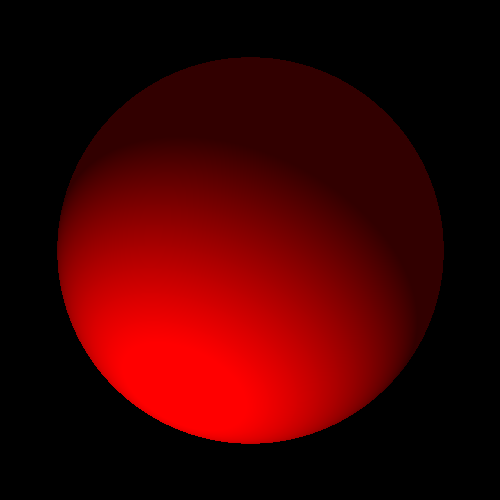
\includegraphics[scale=0.3]{boule.png}
	\caption{\label{fig:sphère} Application d’une lumière diffuse à une sphère rouge \protect \footnotemark }
\end{figure}
\footnotetext{http://linut.free.fr/omgspl0kuberwebloglolz0r/?2010/02/01/93-raytracer-que-la-lumiere-soit}

\paragraph{}
	Pour la création d’un anaglyphe, deux images espacées par une petite distance (qui correspond à la distance entre les deux yeux par exemple) sont générées. La composante rouge de l’une de ces images et la composante bleue de l’autre sont gardées et ensuite superposées dans une même image. Cette image est ensuite transformée en une image Rouge-Cyan, qui peut être visualisée à l’aide de lunettes Rouge-Bleue : l’image apparaît en trois dimensions.

\paragraph{}
	Pour la création d’un autostéréogramme, une image permettant d'observer un objet en relief par vision parallèle est générée. Cette image est obtenue à partir d'une texture de base ou de points aléatoires pour l'image de fond.

\paragraph{}
	Pour la création d’un flipbook, plusieurs images sont prises à intervalles réguliers par une caméra suivant un trajet prédéterminé dans ou autour de la scène. Le flipbook est visualisable en faisant rapidement défiler ces images tout en respectant l’ordre des prises de vue. Ce flipbook peut être transformé en GIF pour obtenir une visualisation animée des images.


\section{Etat de l'art et existant}
\subsection{Logiciels existants}

\paragraph{}
	StereoPhoto Maker \footnote{StereoPhoto Maker : http://stereo.jpn.org/eng/stphmkr/} et Anaglyph Maker 3D \footnote{Anaglyph Maker 3D : http//www.stereoeye.jp/software/index\_e.html} sont des freewares permettant, entre autre, depuis deux photos d'obtenir l’anaglyphe rouge / cyan correspondant. La qualité de l'anaglyphe obtenu dépend du décalage entre les deux photos et de la qualité de la prise de vue. 
	
\paragraph{}
	Enfin, de nombreux logiciels de création d'autostéréogrammes sont disponibles, comme Stereographic Suite  (\copyright IndaSoftware) et 3DMiracles(\copyright Urry Software Lab) qui permettent de créer des autostéréogrammes à partir d'une carte de profondeurs (image en deux dimensions en niveaux de gris).
	
\subsection{Projection vers deux dimensions}

\paragraph{}
	Le passage d’un objet en trois dimensions à une image en deux dimensions se fait par projection. Une caméra présente dans la scène est déterminée par sa position et le vecteur direction qui indique vers quel endroit elle regarde dans la scène [1]. La vue elle-même est obtenue par projection de la scène dans le repère de la caméra comme sur la figure  \ref{fig:projection}.
	
\begin{figure}[h]
		\centering
		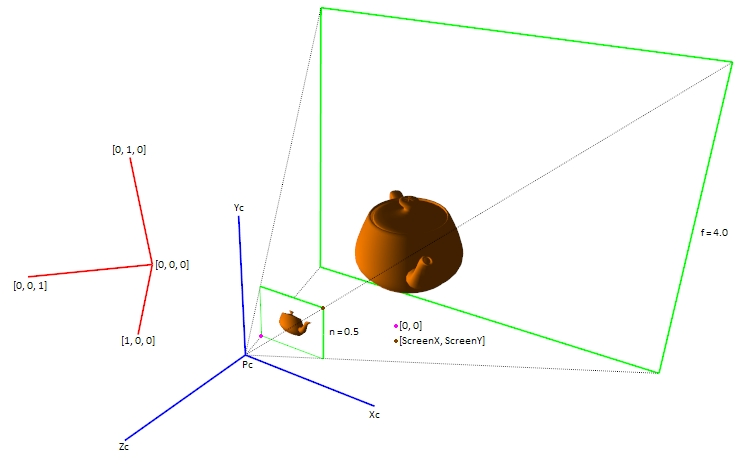
\includegraphics[scale=0.7]{projection.png}
		\caption{\label{fig:projection} Projection d’un objet en trois dimensions sur un support en deux dimensions \protect \footnotemark }
\end{figure}
	\footnotetext{OpenGL perspective projection : http://www.3dcpptutorials.sk/index.php?id=2}
	
\subsection{Les flipbooks}

\paragraph{}
	Le principe d’un flipbook, ou folioscope en français, est de créer une suite d’images successives d’une scène par rapport à une trajectoire. Il suffira ensuite de mettre toutes ces images dans l’ordre les unes derrière les autres, et de les faire défiler rapidement pour avoir l’impression d’un rendu en relief et en mouvement comme sur la figure 3. C’est également le principe des fichiers d’extension .GIF, qui font défiler une liste d’images.
	
\paragraph{}
	La création d’un flipbook est possible en créant une animation à l’aide d’un logiciel de manipulation d’objets 3D et en ne capturant que certaines images, par exemple avec Blender. Ainsi l’impression de ces images successives permet de réaliser un flipbook (cf. figure \ref{fig:flipbook}). En combinant par exemple avec le logiciel Gimp (outil d’édition et de retouche d’image) l’animation peut être obtenue en GIF. 

\begin{figure}[h!]
		\centering
		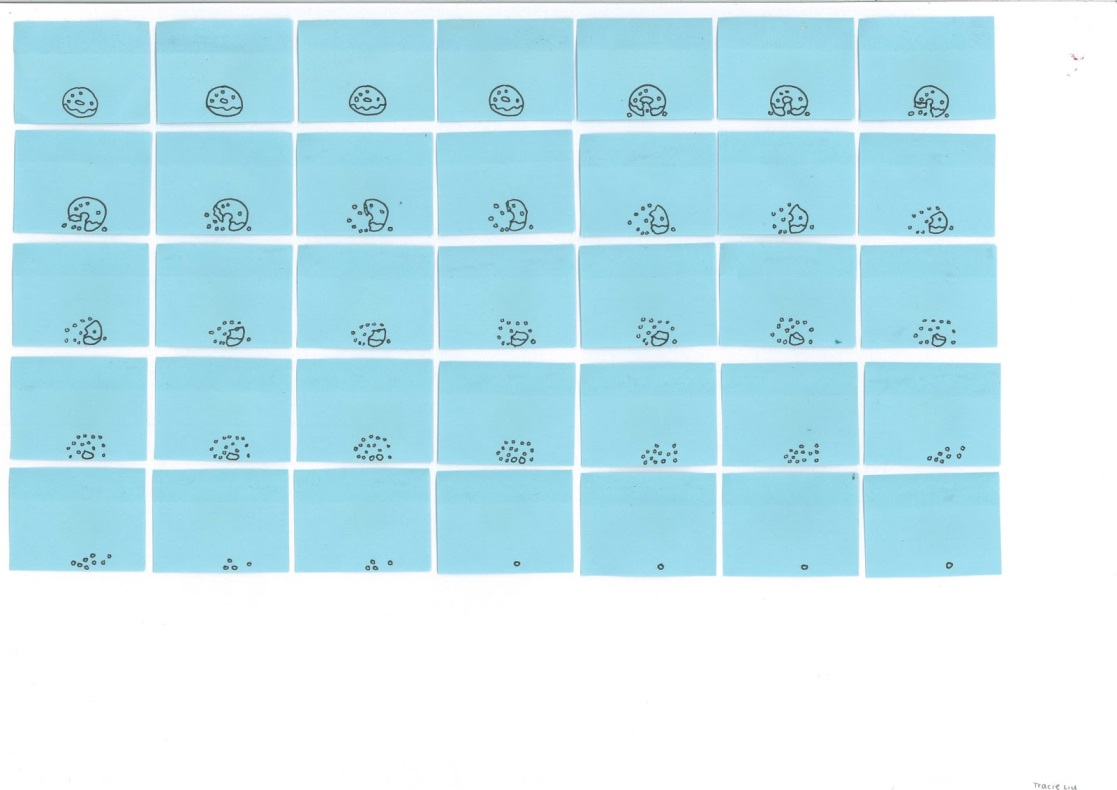
\includegraphics[]{flipbook.png}
		\caption{\label{fig:flipbook} Story-board d’un flipbook \protect \footnotemark }
\end{figure}
\footnotetext{http://tracieliu.blogspot.fr/2010/08/flipbook-storyboard.html}

\subsection{Les autostéréogrammes}	

\paragraph{}
Un autostéréogramme est une image qui cache une visualisation en trois dimensions d’un objet. La visualisation en trois dimensions peut être difficile à obtenir, et demande une réelle gymnastique oculaire. Cette image est construite de sorte qu'à chaque point de l'objet en trois dimensions soient associés deux points de l'image. L'utilisateur doit observer chaque point d'un couple de points avec un seul œil, ce qui donne l'illusion au cerveau d'observer deux images différentes avec les deux yeux et donc l'incite à traiter cette information comme l'observation d'un objet en trois dimensions, comme illustré par la figure \ref{fig:ppe_autostereogramme}.

\begin{figure}[h!]
  \centering
  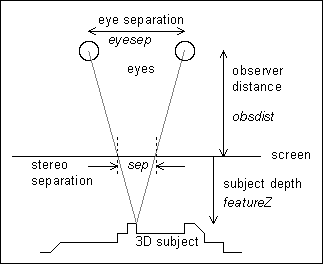
\includegraphics{./ppe_autostereogramme.png}
  \label{fig:ppe_autostereogramme}
  \caption{Visualisation d’un autostéréogramme en vision parallèle \protect \footnotemark }
\end{figure}
\footnotetext{http://www.techmind.org/stereo/geometry.gif}

\paragraph{}
La visualisation en trois dimensions peut être difficile à obtenir, et demande une réelle gymnastique oculaire. Il faut pouvoir fixer le regard en avant ou en arrière de l’image, pour réussir à y voir l’objet caché. La plupart des autostéréogrammes sont observables en vision parallèle, c'est-à-dire qu'il faut faire le point au-delà de l'image pour pouvoir observer l'objet.

\paragraph{}
	Pour générer un autostéréogramme, il faut utiliser une carte des profondeurs, ou carte de disparité, de l’objet à dissimuler. Cette carte s’obtient grâce à deux visions d’une même scène prises à deux endroits différents, et permet de mettre en avant les informations sur la profondeur de l’objet. Par exemple, la carte des profondeurs de la figure \ref{fig:carteProfondeur} a permis d’obtenir l’autostéréogramme de la figure \ref{fig:autostereogramme}.

\begin{figure}[h!]
		\centering
		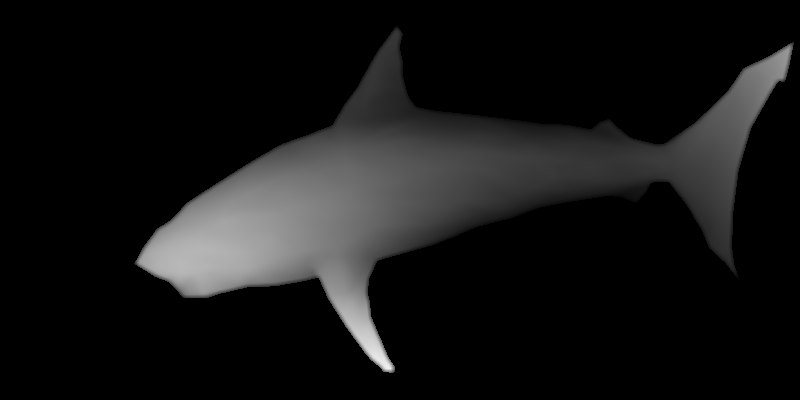
\includegraphics[scale=0.4]{carteProfondeur.png}
		\caption{\label{fig:carteProfondeur} Carte des profondeurs \protect \footnotemark }
\end{figure}
\footnotetext{http://en.wikipedia.org/wiki/Autostereogram}
\begin{figure}[h]
		\centering
		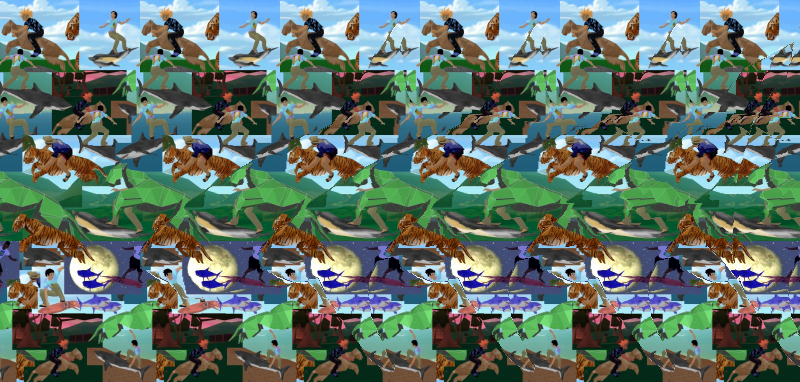
\includegraphics[scale=0.5]{autostereog.png}
		\caption{\label{fig:autostereogramme} Autostéréogramme obtenu \protect \footnotemark }
\end{figure}
\footnotetext{http://en.wikipedia.org/wiki/Autostereogram}

\paragraph{}
Il existe des algorithmes de génération d’autostéréogrammes très simples , comme celui proposé par Gary Beene \cite{garybeene}. Cependant un algorithme aussi peu optimisé produit des autostéréogrammes défecteux, comportant par exemple des échos (répétition d'une partie de l'objet 3D) ou des artefacts (défaut de l'objet 3D observé).

\paragraph{}
Des algorithmes plus poussés ont été développés, comme celui présenté par Harold W. Thimbleby, Stuart Inglis et Ian H. Witten \cite{stereogram}, et celui proposé par W. A. Steer \cite{wasteer}, associés à une réalisation en C. Ils permettent la génération d’autostéréogrammes SIRDS (Single Image Random Dots Stereogram) à partir d’une image 2D. Ces articles présentent également des méthodes de correction de problèmes tels que l'écho ou la gestion des faces cachées (faces de l'objet tridimensionnel visibles par un seul œil). W. A. Steer propose de plus une méthode de génération d'autostéréogrammes utilisant un motif bitmap comme image de base plutôt qu'un nuage de points aléatoires, ce qui pallie à certaines limites des SIRDS comme le manque de détails et la grossièreté des surfaces courbes.


\subsection{Les anaglyphes}

\paragraph{}
	Un anaglyphe est une image sur laquelle on superpose deux vues, si possible différentes, d’une scène. La meilleure distance entre ces deux visions est la même que celle entre les deux yeux, afin que le cerveau puisse recréer la même vision en trois dimensions que dans la réalité.
	
\paragraph{}
	Les anaglyphes les plus fréquents sont les anaglyphes dits rouge-cyan. Ils se nomment ainsi car ils sont constitués d’une image sur laquelle on passe un filtre magenta, et une autre avec un filtre cyan (cf. figure \ref{fig:anaglyph}). Pour pouvoir visualiser le relief sur une telle image, on utilise une paire de lunettes rouge-cyan, dont chaque verre est un filtre pour l’une des deux couleurs de l’image. Le plus souvent, le filtre magenta est placé sur l’œil gauche, le cyan sur l’œil droit. En regardant l’image, l’œil gauche ne verra alors que la composante cyan, et inversement pour l’œil droit. Les deux images ayant un léger décalage, le cerveau va percevoir l’image comme si elle était en trois dimensions. Les anaglyphes rouge-cyan sont principalement intéressants sur des images en noir et blanc. En effet, quand il s’agit d’images en couleur, celles-ci sont souvent détériorées par l’usage des filtres, car les couleurs sont généralement composées de plusieurs composantes. A l’inverse, quand l’image est en nuances de gris, l’image n’est pas modifiée, juste mise en relief.

\begin{figure}[h]
		\centering
		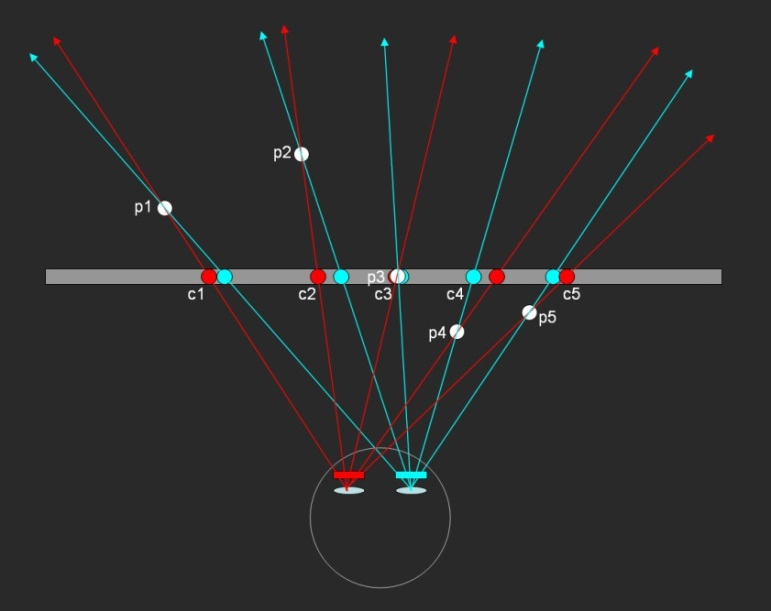
\includegraphics[scale=1]{anaglyph.png}
		\caption{\label{fig:anaglyph} Le décalage de la partie rouge et cyan permet à l’œil de percevoir l’image non plus dans un plan XY mais dans l’espace \protect \footnotemark }
\end{figure}
\footnotetext{http://www.david-romeuf.fr/3D/Anaglyphes/TCAnaglypheLSDubois/TransformationCouleursPourAnaglyphe.html}

\paragraph{}
	Le paragraphe précédent concernent la création d’un anaglyphe depuis deux prises de vue d’une même scène avec un léger décalage. Mais il est également possible de le faire à partir d’une image en deux dimensions grâce à l’algorithme de Dubois \cite{algoDubois}, qui définit une vision matricielle de l’anaglyphe (cf. figure \ref{fig:algoDubois}). Dès lors, une matrice de transformation est introduite, qui permet de passer du taux RGB d’un pixel de l’image originale,  aux deux taux RGB des anaglyphes gauche/droite. Les coefficients de cette matrice sont calculés pour satisfaire une bonne restitution de l’image originale, tout en supprimant les rivalités colorées induites par des lunettes bicolores. Ainsi, pour visualiser une image rouge pure, il faudra changer le taux RGB de ce pixel pour que les deux yeux puissent le voir après les filtres. Sinon l’information ne circulera que dans un œil, et l’on perdra la vision stéréoscopique, et donc la notion de profondeur. 
	
\begin{figure}[h]
		\centering
		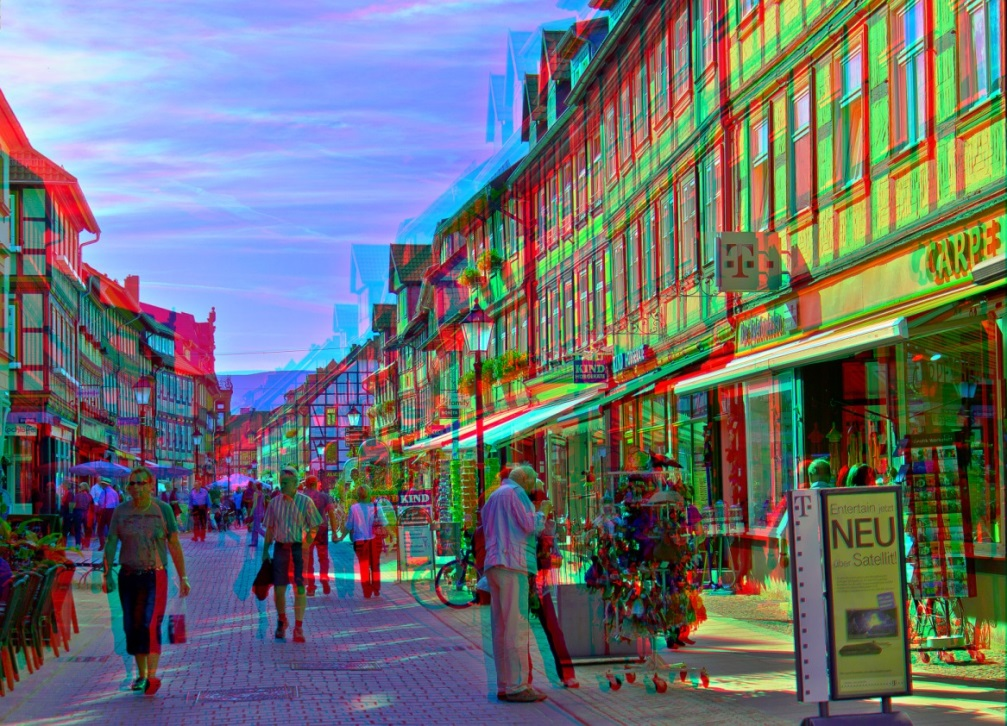
\includegraphics[scale=1]{algoDubois.png}
		\caption{\label{fig:algoDubois} Rendu final d’une image par l’algorithme de Dubois \protect \footnotemark }
\end{figure}
\footnotetext{http://zour.deviantart.com/art/Wernigerode-Boulevard-Dubois-Anaglyph-HDR-3D-276542278}
	
	


\section{Sujet}
présentation du sujet
reprendre présentation du cahier des charges
améliorer avec une vision plus poussée du projet

\paragraph{}
	Le projet concerne la réalisation d’un logiciel permettant d’obtenir des projections en deux dimensions, des anaglyphes, des autostéréogrammes ou encore des flipbooks à partir de scènes virtuelles en trois dimensions. 

\paragraph{}
	L’objectif premier est de permettre la visualisation, sur un support en deux dimensions tel qu’un écran d’ordinateur ou une feuille de papier, d’un espace en trois dimensions. A partir de la visualisation d’objets 3D dans une scène il faudra donc réaliser des photographies qui une fois traitées donneront lieu à des anaglyphes, autostéréogrammes ou des animations type flipbook.
	
\paragraph{}
	Afin d’atteindre cet objectif, un logiciel s’appuyant sur le moteur 3D OpenGL devra être réalisé. Il permettra la création d’une scène où s’inséreront des objets dont la position, la taille et l’orientation seront paramétrables. Une caméra permettra de se déplacer dans la scène, de s’en rapprocher ou s’en éloigner.

\paragraph{}
	Une fois la scène mise en place, il faudra pouvoir prendre des photographies de celle-ci sous différents angles afin d’obtenir, après application d’algorithmes de traitement d’images :

\begin{itemize}
	\item
		des anaglyphes rouge-cyan, qui permettront une visualisation en trois dimensions grâce à des lunettes adaptées ;
	\item
		des stéréogrammes, qui sont des images dissimulant un contenu qui apparaît quand on fixe le dessin de façon spécifique ;
	\item
		des flipbooks ou images animées, correspondant à une succession d’images suivant une trajectoire qui permettent en les faisant défiler de donner une impression de mouvement.
\end{itemize}


\section{Cahier des besoins}
\subsection{Besoins fonctionnels}
\subsection{La scène}
Cette partie montre l’ensemble des cas d’utilisation relatifs à la scène.

\begin{description}[style=nextline]
    \item[Création de la scène]
    \mbox{\hspace{1cm}} Au démarrage du logiciel, il sera possible de créer une nouvelle scène ou d’en charger une préexistante. Celle-ci permettra d’afficher et disposer plusieurs objets 3D avant d’être sauvegardée pour une utilisation ultérieure.
    
    \item[Sauvegarde de la scène] 
    \mbox{\hspace{1cm}} On distinguera deux types de sauvegardes indépendantes entre elles : la sauvegarde automatique et la sauvegarde manuelle. La première s’effectuera après chaque modification apportée avec pour but d’éviter la perte de données en cas de crash du logiciel, elle se fera de manière discrète (c’est à dire en arrière-plan sans figer le logiciel le temps de la sauvegarde). La seconde se fera au format XML (dont le prototype est détaillé ultérieurement) sur demande de l’utilisateur. Il sera possible de choisir entre une importation des objets utilisés dans le répertoire courant de la scène ou d’une simple sauvegarde des chemins d’accès aux modèles 3D. Par ailleurs, les deux types de sauvegarde étant indépendants, une sauvegarde manuelle n’écrasera pas une sauvegarde automatique.
    
    \item[Chargement de la scène] 
    \mbox{\hspace{1cm}} Comme vu précédemment, lors de la sauvegarde, les données relatives aux objets de la scène seront stockées dans un fichier au format XML. A l’ouverture du logiciel, l’utilisateur pourra choisir d’ouvrir une scène qu’il aura sauvegardée précédemment. Dans ce cas, les données enregistrées seront récupérées pour recréer la scène telle qu’elle était avant la fermeture du logiciel.
    
    \item[Suppression de la scène]
    \mbox{\hspace{1cm}} Le logiciel ne proposera pas directement de méthode pour supprimer une scène. Pour cela, il faudra directement aller supprimer le dossier associé à la sauvegarde à l’intérieur du dossier contenant le logiciel.
    
\end{description}
	
\subsection{Les objets}
Une fois la scène créée ou chargée, l’utilisateur aura la possibilité d’y placer des objets.

\begin{description}[style=nextline]
	\item[Chargement des fichiers objets]
	\mbox{\hspace{1cm}} Les objets en trois dimensions utilisés seront sous la forme de fichiers objets. Trois types seront acceptés : les fichiers d’extension .OBJ (version 3.0, ASCII) et .PLY (versions 1.0, ASCII et binaire). Ils devront permettre de définir des objets à facettes triangulaires. Les objets pourront être ceux de l’utilisateur ou de la bibliothèque implémentée dans le logiciel. \newline
	\mbox{\hspace{1cm}}Ces objets ne devront contenir aucun trou, par exemple une face absente sur un cube ou un triangle non généré par le fichier de chargement. Le fonctionnement du logiciel n’est garanti que sur des objets topologiquement valides. \newline
	\mbox{\hspace{1cm}}Si un fichier à charger possède trop de polygones, un algorithme de décimation de faces permet d’en réduire le nombre jusqu’à un certain seuil (cf. prototype). Ce traitement n’est pas automatique et l’utilisateur pourra ou non l’appliquer.
	
	\item[Placement d'un objet]
	\mbox{\hspace{1cm}} Après le chargement de l’objet il sera possible de le placer dans la scène via les trois translations du repère 3D. Ce placement n’est pas définitif et pourra être modifié ultérieurement lors de la constitution de la scène.
	
	\item[Modification d'un objet]
	\mbox{\hspace{1cm}}Trois caractéristiques d’un objet pourront être modifiées : son emplacement, son orientation et sa taille.
	
	\item[Modification de l'orientation d'un objet]
		\mbox{\hspace{1cm}}	L’orientation d’un objet dans la scène pourra être modifiée en fonction des trois axes de rotation usuels.
	
	\item[Modification de la taille d'un objet]
		\mbox{\hspace{1cm}} L’objet pourra être agrandi ou réduit selon le besoin.
		
	\item[Mode de modification d'un objet]
	\mbox{\hspace{1cm}}	Le placement et le paramétrage de l’objet (orientation, taille …) n’est pas définitif et peut-être revu par la suite via un mode de modification après avoir sélectionné l’objet à modifier. Toute sortie de ce mode de modification entraînera une sauvegarde automatique de la scène. 
		
	\item[Sélection d'un objet]
	\mbox{\hspace{1cm}} Il sera possible de sélectionner un objet pour réaliser des modifications.
	
	\item[Suppression d'un objet]
	\mbox{\hspace{1cm}} Il sera également possible, après sélection, de supprimer un ou plusieurs objets de la scène. Le ou les objets ainsi supprimés ne seront plus référencés dans la sauvegarde.
\end{description}		


\subsection{La caméra}
La caméra possède un repère qui lui est propre et une distance correspondant à celle entre l’origine du repère de la scène (centre de rotation de la caméra) et le sien. 

	
\begin{description}[style=nextline]
	\item[Observation de la scène]
	\mbox{\hspace{1cm}}La caméra permettra de se déplacer dans la scène en suivant les trois axes de rotation et les trois axes de translation usuels, ainsi qu’un zoom. Si l’on choisit de se déplacer relativement aux axes de translation, le centre de rotation de la caméra sera modifié.

	\item[Type de projection]
	\mbox{\hspace{1cm}}	Deux types de projections seront disponibles : la projection orthographique (qui sera l’option par défaut) et la projection en perspective.

	\item[Zoom de la scène]
	\mbox{\hspace{1cm}}Il sera possible de se rapprocher ou s’éloigner de la scène via une fonctionnalité de zoom. Il ne sera pas possible d’atteindre le centre de rotation de la caméra.

	\item[Remise à zéro du centre de la caméra]
	\mbox{\hspace{1cm}}La position de la caméra pourra, à tout moment, être réinitialisée pour se retrouver dans les conditions initiales de visionnage de la scène.
	
\end{description}

\subsection{Le passage en deux dimensions}
\begin{description}[style=nextline]
	\item[Mode de passage en deux dimensions]
	Différents rendus seront accessibles : 
	\begin{itemize}
			\item Photographie
			\item Anaglyphe noir et blanc via un algorithme améliorant le rendu post-impression ou s’appliquant sur des paires d’images pseudo stéréoscopique.
                        \item Flipbook d'une rotation autour d'un objet ou d'une scène.
	\end{itemize}
	Pour les images générées par les modes présentés ci-dessous, il faudra choisir entre une qualité de 75 ou 300 pixels par pouce. \colorbox{yellow}{Préciser les algorithmes} 
	
	\item[Mode photographie]
	\mbox{\hspace{1cm}} Le mode photographie permettra d’obtenir une image proche de la scène virtuelle créée. Pour ce mode, des informations concernant la qualité de l’image et sa taille devront être fournies.
	
	\item[Mode analgyphe]	
	\mbox{\hspace{1cm}}Le mode anaglyphe permettra d’obtenir une image rouge, une image cyan, ainsi qu’une image superposant les deux. Pour ce mode, des informations concernant la qualité de l’image et sa taille devront être fournies.
	
	\item[Mode autostéréogramme]	
	\mbox{\hspace{1cm}}Le mode autostéréogramme permettra d’obtenir un autostéréogramme fixe à une image. Pour ce mode, des informations concernant la qualité de l’image et sa taille devront être fournies.
	
	\item[Mode flipbook]	
	\mbox{\hspace{1cm}}Le mode flipbook permettra d’obtenir un ensemble d’image sur une trajectoire donnée. Pour ce mode, des informations concernant la qualité de l’image et sa taille, mais également des informations nécessaires au lancement et à la construction du flipbook devront être fournies par l’utilisateur. Ainsi, il devra tout d’abord choisir une trajectoire parmi les trois axes de rotation, les trois axes de translation ou le zoom, puis un point de départ. Au choix, il pourra alors sélectionner un point d’arrivée et un nombre d’images, ou un nombre d’image et un angle pour connaître la mesure entre deux prises. Une barre de progression indiquera le nombre prises de vues faites par rapport au total. Si le temps d’attente est trop long, il sera toujours possible d’annuler l’action et redéfinir les paramètres.
	
	\item[Affichage du rendu]
	\mbox{\hspace{1cm}}Les algorithmes des modes présentés ci-dessus permettront d’obtenir un rendu correspondant aux attentes de l’utilisateur. Ce dernier sera ensuite affiché dans une nouvelle fenêtre contenant le ou les produits demandé qu’il sera possible de sauvegarder avant de quitter.
	
	\item[Enregistrement du rendu]
	\mbox{\hspace{1cm}} Si l’utilisateur choisit d’enregistrer les images générées par les algorithmes, les rendus qu’il souhaite sauvegarder devront être choisis parmi les rendus obtenus.
	
	\item[Enregistrement de la photographie]
	\mbox{\hspace{1cm}}	Pour le cas simple de la photographie, il faudra nommer le fichier et donner son emplacement avant qu’il ne soit enregistré au format PNG.
	
	\item[Enregistrement de l'anaglyphe]
	\mbox{\hspace{1cm}} Les images rouge et cyan pourront être enregistrées séparément ou non. Deux options de rendus seront disponibles : pour l’impression et pour l’ordinateur. Elles permettront d’optimiser l’affichage et l’utilisation des lunettes dans les deux cas. 
	
	\item[Enregistrement de l'autostéréogramme]
	\mbox{\hspace{1cm}}	Pour l' autostéréogramme, il faudra nommer le fichier et indiquer son emplacement avant de le sauvegarder au format PNG.
	
	\item[Enregistrement du flipbook]
	\mbox{\hspace{1cm}}Dans le cas du flipbook, les images pourront être enregistrées une à une au format PNG, par tranche au format PNG ou sous forme d’animation GIF. Dans le cas d’une sauvegarde séparée de chaque image il faudra les nommer et donner leur chemin d’accès. Par tranche il faudra indiquer la première et la dernière image ainsi qu’un nom commun et un répertoire. Pour l’animation il faudra la nommer et donner son chemin d’accès. 
\end{description}

\subsection{Besoins non fonctionnels}
\subsubsection{La fluidité d'affichage}
\paragraph{}
	Pour que l’affichage soit fluide la machine devra avoir au minimum 2Go de mémoire vive, un processeur récent avec au moins 2 cœurs cadencés au minimum à 2GHz et les conditions suivantes devront être validées :

	\begin{itemize}
		\item 
		Pour une machine avec processeur graphique type Intel HD Graphics 4000 ou plus récent, au maximum 100 000 points pour un affichage à 25 fps, ou 150 000 points pour un affichage à 20 fps ;
		\item
		Pour une machine avec une carte graphique type NVIDIA GTX 720 ou plus récente, au maximum 350 000 points pour un affichage à 25 fps, ou 500 000 points pour un affichage à 20 fps.
		
	\end{itemize}
	
\textbf{\underline{Test de validation}} : ouverture de plusieurs modèles 3D, présentés en annexe, dans Meshlab sur différentes machines. Les résultats sont également disponibles en annexe.

\subsubsection{Fluidité d'obtention des rendus}
\paragraph{}
	A l’heure actuelle on ne peut garantir un nombre de points assurant l’obtention d’un rendu en un temps raisonnable. C’est pourquoi une barre de progression s’affichera pour que l’utilisateur ait une idée du temps d’attente avant l’affichage du résultat.

\subsubsection{Portabilité du logiciel}
\paragraph{}
La portabilité rend le logiciel accessible à un plus grand nombre de personnes. Les systèmes d’exploitation visés seront Windows XP, Windows Seven, Windows 8.1, Ubuntu 14.04, Fedora 20 et Debian Jessie, en plateforme 32 bits et 64 bits. \newline

\textbf{\underline{Test de validation}} : un prototype, qui pourra être utilisé comme base du projet, a été exécuté sur l’ensemble de ces systèmes d’exploitation (cf.  la partie \ref{sec:prototypetest} Prototype test).

\subsubsection{Extensibilité du logiciel}
\paragraph{}
	Le client souhaite que l’extensibilité du logiciel soit facilitée par son architecture. En effet, il envisage par la suite d’ajouter de nouvelles fonctionnalités ou de nouveaux algorithmes au logiciel, et demande à ce que de telles modifications soient aisément envisageables.
\paragraph{}
	La facilitation de cette extensibilité sera permise par l’utilisation d’une architecture spécifique. Celle-ci est détaillée dans la partie \ref{sec:archi} Architecture du projet de ce cahier des charges.   

\subsection{Contraintes}
\subsection{Superposition des objets dans la scène}

\paragraph{}
	Pour faciliter le traitement d’une scène, on considèrera que deux objets placés dans une scène ne pourront pas être superposés. On parle ici d’intersection des boîtes englobant des objets et non de la gestion des parties non visibles des objets lors de l’affichage.

\subsection{Utilisation des bibliothèques}

\paragraph{}
	Afin de minimiser les dépendances et valider le besoin en portabilité les bibliothèques Qt et OpenGL seront utilisées. CMake permettra de générer les scripts de compilation quel que soit la plateforme.
	
\subsection{Langage de programmation}

\paragraph{}
	Le langage C++ sera utilisé.

\subsection{Open Source}

\paragraph{}
	Pour permettre l’utilisation du logiciel et son extensibilité à quiconque souhaiterait le modifier, on choisira de laisser le code du projet en Open Source. Pour garantir cela, on s’assura bien que l’on dispose des droits nécessaires pour n’importe quel algorithme ou fragment de code utilisé au cours de ce projet.
	
\subsection{Briques logicielles}
\subsection{Meshlab}

\paragraph{}
	En développement depuis 2005, Meshlab est un logiciel libre de traitement de maillage 3D disponible sur Microsoft Windows, Mac OS X, GNU / Linux et ses dérivés. Il propose différents outils comme des filtres de nettoyage du maillage, la possibilité de supprimer le bruit etc. C’est un logiciel très apprécié dans le domaine universitaire pour la reconstruction de surface, l’impression 3D etc. car il s’agit d’un logiciel non seulement gratuit, mais également Open Source. Cela permet d’avoir une base commune et grâce à une communauté active, de nouvelles fonctionnalités peuvent être ajoutées et utilisées par tout le monde. 

\subsection{Blender}

\paragraph{}
	Blender est, depuis 2003, un logiciel libre de modélisation, d’animation et de rendu 3D disponible sur de nombreuses plateformes comme Microsoft Windows, Mac OS X, GNU / Linux et ses dérivés. C’est un logiciel extensible,  léger, ne réclamant pas un ordinateur très puissant pour des actions simples. Sa communauté de fan très développée a permis la réalisation d’une base de données de greffons conséquente. Preuve de sa puissance, celui-ci a été utilisé pour réaliser entièrement un film d’animations (Tears of Steel) et pour les effets spéciaux de plusieurs films tels que Mr. Nobody.
	


\section{Maquette}
Cette partie montrera l’ensemble des maquettes de la future interface du logiciel.

\subsection{Fenêtre principale}

\begin{figure}[H]
  \centering
  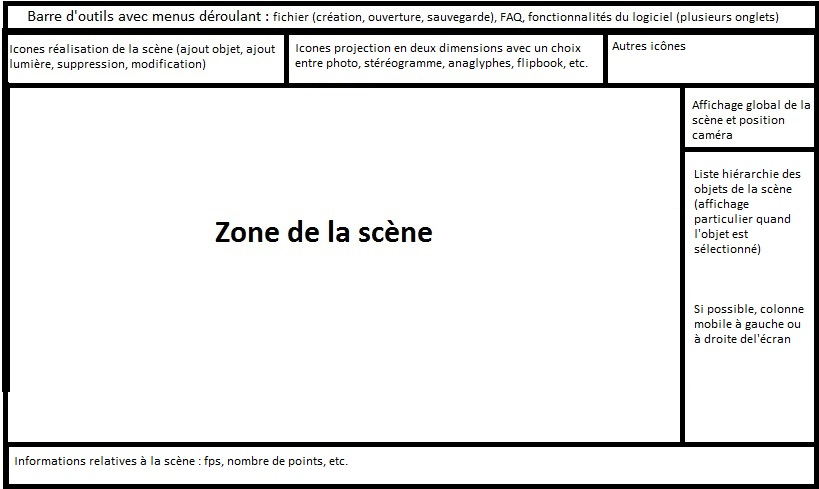
\includegraphics[scale=0.6]{fenetreprincipale}
  \caption{Fenêtre principale}
  \label{fig:fenppale}
\end{figure}

La fenêtre principale (\ref{fig:fenppale}) se détaille comme suit :

\begin{itemize}
\item Barre d'outils avec menus déroulants
  
  Ce bandeau supérieur correspond à un bandeau supérieur de logiciel classique, comme on le trouve par exemple dans le logiciel Meshlab.

  L’intérêt de ces menus déroulants est de proposer l’accès à l’ensemble des fonctionnalités du logiciel. Parmi ces menus se trouvent quelques redondances avec des icônes présentes dans d’autres parties de la fenêtre principale, afin que l’utilisateur puisse choisir l’utilisation du logiciel qui lui convient le mieux.
  
\item Icônes de réalisation de la scène
  
  Les icônes permettant de réaliser la gestion des objets et des lumières de la scène : il sera possible d’ajouter un objet ou de le modifier à partir de ces icônes.

\item Icônes de projection en deux dimensions
  
  L’ensemble des icônes permettant d’obtenir l’un des rendus possibles à l’aide du logiciel, c’est-à-dire quatre icônes pour : une projection en deux dimensions classique, la création d’un anaglyphe, la création d’un stéréogramme et la création d’un flipbook.
  
  L’ensemble de ces icônes permettra d’ouvrir une nouvelle fenêtre et de choisir les paramètres de l’image à obtenir.

\item Autres icônes
  
  Cette zone pourra contenir d’autres icônes, qui seront triées et rassemblées en fonction de leurs cas d’utilisation.

\item Zone de la scène
  
  Vu de la scène du point de vue de la caméra. L’utilisateur pour s’y déplacer librement via la caméra pour pouvoir l’observer depuis différents angles. Il pourra également sélectionner des objets pour les déplacer, modifier leur orientation, les redimensionner ou les supprimer.

\item Liste des objets de la scène
  
  L’ensemble des objets présents dans la scène listés : l’utilisateur pourra cliquer sur le nom d’un objet afin de le sélectionner et de pouvoir agir dessus.

\item Informations relatives à la scène
  
  Des informations intéressantes pour l’utilisateur par rapport à la scène et à son affichage seront affichées : le nombre d’objets dans la scène, le nombre de points, ou encore la qualité d’affichage en frames par seconde. Cette zone pourra également servir à l’affichage de messages informatifs ou de messages d’erreurs à l’intention de l’utilisateur.
\end{itemize}

\subsection{Fenêtre d'affichage du rendu}

\begin{figure}[H]
  \centering
  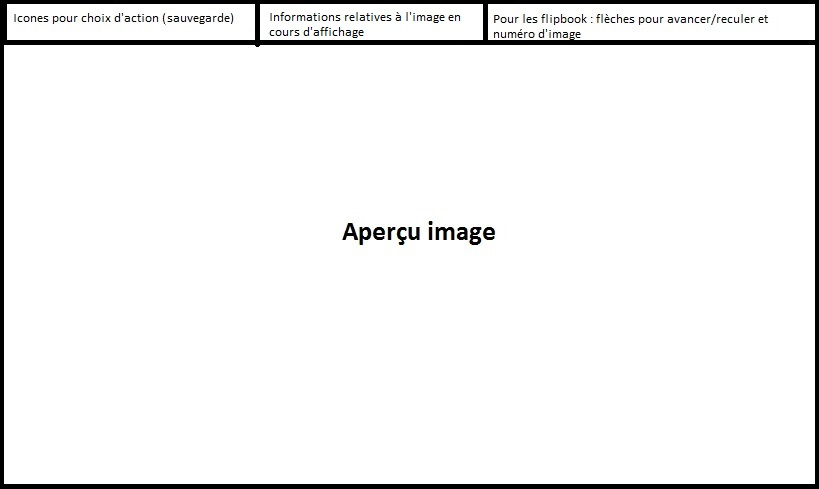
\includegraphics[scale=0.6]{apercuimage}
  \label{fig:apercu}
  \caption{Affichage du rendu}
\end{figure}

\begin{itemize}
\item Zone de choix d’action
  
  Cette zone contiendra des icônes pour indiquer à l’utilisateur les choix qui s’offrent à lui. On trouvera par exemple une icône pour l’enregistrement du rendu, qui ouvrira une nouvelle fenêtre pour laisser le choix à l’utilisateur de ce qu’il souhaite enregistrer.
  
\item Zone d’affichage des informations
  
  Cette zone concernera uniquement l’image en cours d’affichage dans la zone d’aperçu. On détaillera ici la taille de l’image et sa qualité en pixels par pouce.
  
\item Zone de défilement
  
  Cette zone contiendra des flèches de déroulement vers la gauche ou vers la droite pour permettre à l’utilisateur de voir l’ensemble des images obtenues, ainsi qu’un ou plusieurs boutons pour pouvoir afficher un GIF ou le stopper.
  
\item Zone d’aperçu de l’image
  
  S’affichera ici l’image obtenue après la requête d’un utilisateur.
  
\end{itemize}


\subsection{Fenêtre de choix des options du rendu}

\begin{figure}[h]
  \centering
  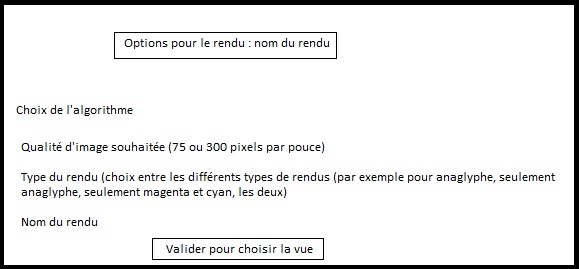
\includegraphics[scale=0.6]{choixoptionsrendu}
  \label{fig:optionsrendu}
  \caption{Choix des options du rendu}
\end{figure}

\paragraph{}
Cette fenêtre s’ouvre lorsque l’utilisateur clique sur le bouton de création d’une projection, d’un anaglyphe, d’un autostéréogramme ou d’un flipbook. Il devra alors choisir l’algorithme à utiliser pour le rendu souhaité (un ou plusieurs algorithmes pourront être proposés), la qualité d’image qu’il souhaite obtenir, ainsi que les types de retour qu’il souhaite obtenir si plusieurs choix existent. Par exemple, dans le cas d’un anaglyphe, le retour pourra contenir ou bien uniquement l’anaglyphe, ou bien les deux vues rouge et cyan, ou bien les deux.

\paragraph{}
L’utilisateur choisira ensuite le nom du rendu et appuiera sur le bouton ``Valider'' pour passer en mode de sélection de la vue. Ce mode reviendra sur la fenêtre principale du logiciel, et des informations seront données à l’utilisateur pour sélectionner la vue qu’il souhaite.

\paragraph{}
Toutes les informations seront obligatoirement complétées pour pouvoir accéder au mode de sélection de la vue.

\subsection{Fenêtre de chargement d'un objet}

\begin{figure}[h]
  \centering
  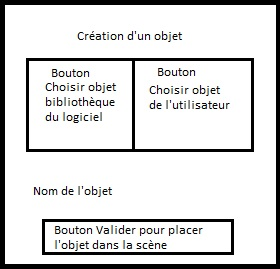
\includegraphics{chargement}
  \label{fig:chargement}
  \caption{Fenêtre de chargement d'un objet}
\end{figure}

\paragraph{}
Pour la création d’un nouvel objet, l’utilisateur du logiciel doit d’ores et déjà avoir ouvert une scène. Il pourra ensuite choisir d’y insérer un nouvel objet grâce à la fenêtre ci-dessus, en choisissant un modèle à ouvrir ainsi que le nom de l’objet dans la scène.

\paragraph{}
Pour le choix du modèle 3D, l’utilisateur pourra utiliser soit la bibliothèque du logiciel soit ses propres fichiers. Toutefois, seules les extensions OBJ, STL et PLY seront acceptées.

\paragraph{}
Une fois toutes les informations entrées, l’utilisateur pourra cliquer sur le bouton Valider pour passer en mode Modification de l’objet et placer son objet dans sa scène.


\subsection{Interface de modification d'un objet}


\begin{figure}[h]
  \centering
  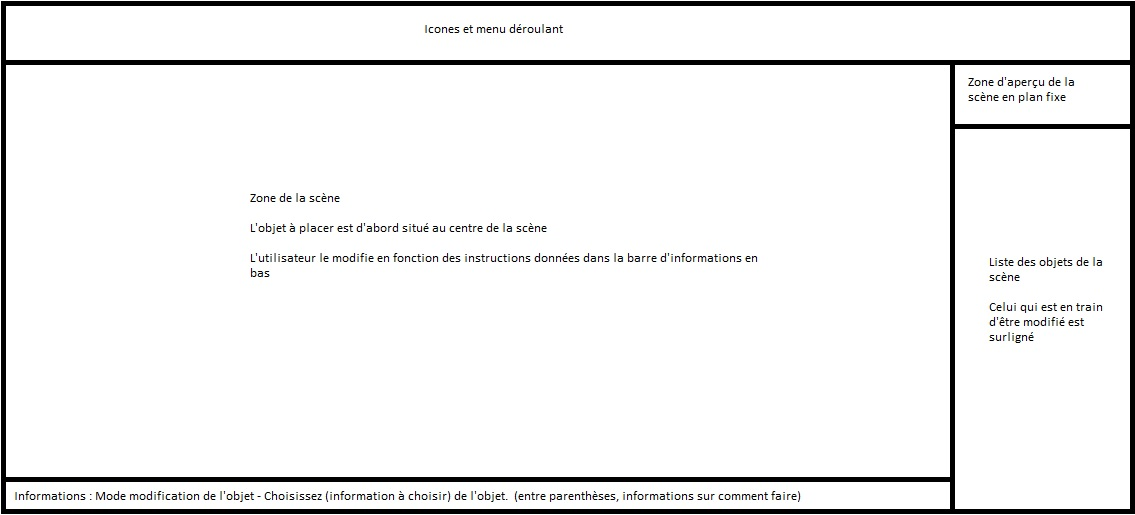
\includegraphics[scale=0.5]{interfacemodifs}
  \label{fig:interfacemodifs}
  \caption{Interface de modification d'un objet}
\end{figure}

\paragraph{}
Une fois qu’il aura choisi le modèle à placer, l’utilisateur verra de nouveau la fenêtre principale s’afficher, et devra suivre les informations indiquées dans la barre Informations en bas de la fenêtre pour modifier la position, l’orientation et la taille de l’objet.

\paragraph{}
S’il souhaite de nouveau effectuer des modifications sur son objet, il devra repasser en mode Modification de l’objet, et retrouvera la même interface que ci-dessus. Il devra à chaque fois obligatoirement passer par les trois modes de modification : position, orientation, taille.


\section{Prototype test}
\subsection{Format de sauvegarde d'une scène}

La sauvegarde d’une scène se fera au format XML. La racine scène contiendra une suite d’objets, une lumière et une caméra. Un objet aura pour attribut son format et son répertoire d’accès et sera caractérisé par une translation, une rotation et un redimensionnement. Une lumière sera directionnelle ou ponctuelle et caractérisée par une couleur, une translation et une rotation. La caméra sera caractérisée par une translation, une rotation et un zoom et une ouverture. Le fichier sera validé par un schéma XML tout au long de la phase de développement et lu via des requêtes XPath.

\paragraph{}
Le schéma XML ainsi qu’un fichier XML de test ont été réalisés et sont disponibles en annexe.

\subsection{Test de fluidité}

Le logiciel Meshlab a été utilisé sur différentes machines avec différents modèles 3D pour déterminer un rapport FPS / nombre de points convenable. Les modèles 3D utilisés contiennent entre 40000 et 14 millions de points.

\subsection{Test de portabilité}

Pour s’assurer de la portabilité de QT et OpenGL sur Windows et Linux, un affichage simple d’un modèle 3D dans une fenêtre QT, sans colorations de face, a été fait et testé sur différentes distributions (fig. \ref{fig:proto_win7}). Les versions 5 de QT et 3.3 d’OpenGL ont été utilisées pour ce prototype et seront utilisées dans la suite du projet. Il a été testé avec des modèles de Stanford comme le dragon, le lapin ou le bouddha.

\begin{figure}[h]
		\centering
		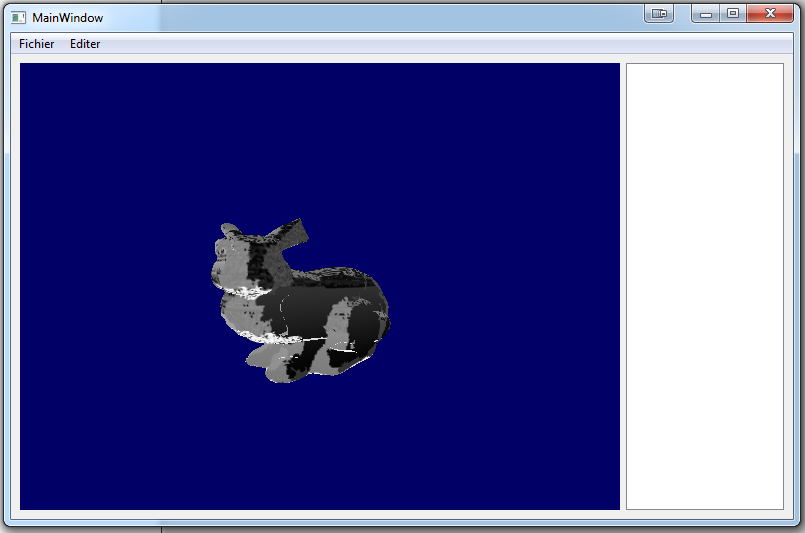
\includegraphics[scale=0.4]{proto_lapin_win7.png}
		\caption{\label{fig:proto_win7} Affichage du modèle 3D de lapin sur Windows 7 }
\end{figure}

\subsection{Réduction du nombre de polygones d’un modèle 3D}

Un algorithme permet de réduire le nombre de faces d’un modèle 3D qui en possèderait trop et serait donc impossible à afficher. Il supprime des triangles et fusionne les sommets autour, jusqu’à ce que le nombre de polygones tombe en dessous d’un certain seuil (fig. \ref{fig:poly_reduc}).
\begin{figure}[h]
		\centering
		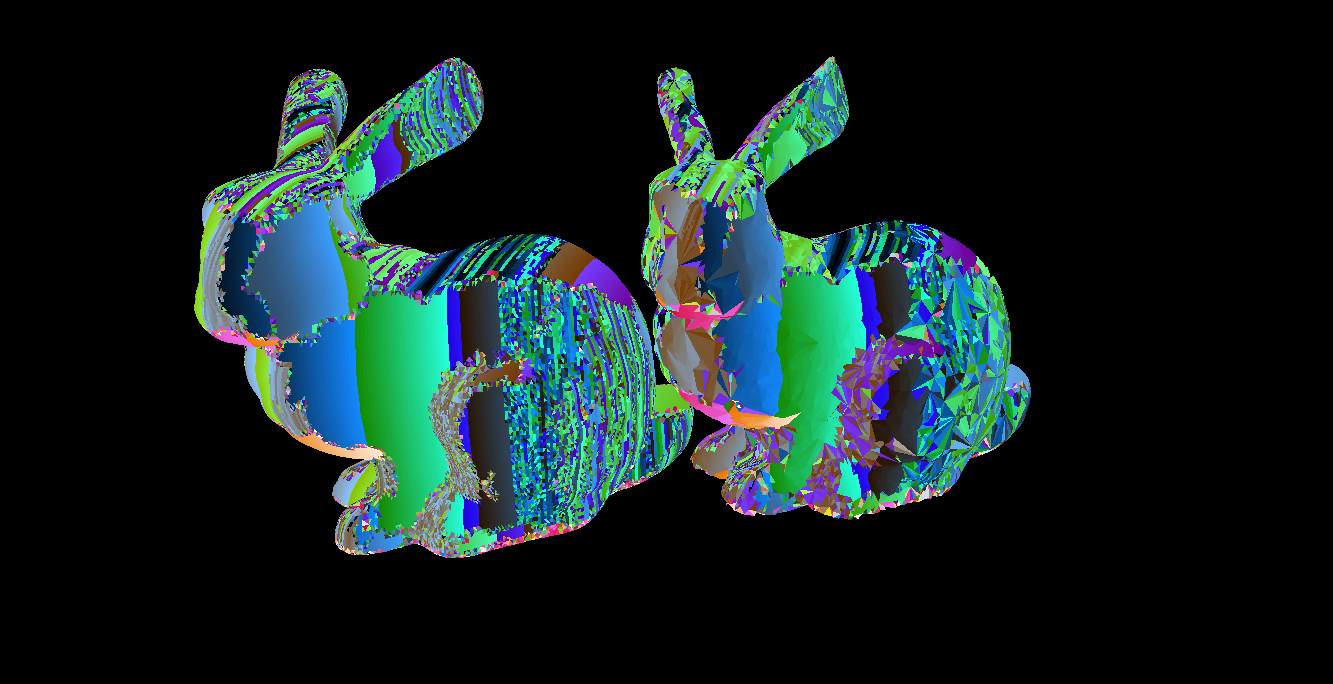
\includegraphics[scale=0.4]{polygon_reduction.png}
		\caption{\label{fig:poly_reduc} \`A gauche modèle 3D d'origine, à droite modèle après suppression de faces }
\end{figure}

\paragraph{}
Ce traitement est effectué lors du chargement et est relativement rapide pour les objets (fig. \ref{fig:poly_reduc_console}).
\begin{figure}[h]
		\centering
		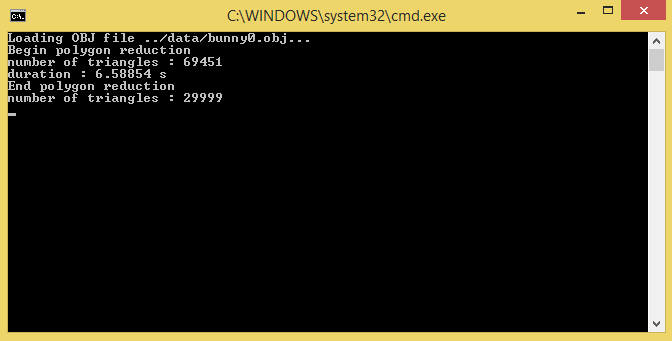
\includegraphics[scale=0.4]{polygon_reduction_console.png}
		\caption{\label{fig:poly_reduc_console}Un test effectué avec l'algorithme sur le modèle de la figure \ref{fig:poly_reduc} montre qu'il met moins de 7 secondes pour supprimer 40000 faces}
\end{figure}


\section{Architecture du projet}
Dans cette partie, nous présenterons un ensemble de diagrammes de séquences et de diagrammes de classes présentant le fonctionnement prévisionnel du logiciel et l’architecture qui en découle. Cette architecture tiendra compte du besoin d’extensibilité du logiciel.

\paragraph{}
Puisque le logiciel disposera d’une interface graphique, c’est par elle que passeront toutes les demandes de l’utilisateur et les rendus qu’il demande.

\paragraph{}
L’ensemble des diagrammes de séquence et des diagrammes de classe présentés par la suite auront été créés grâce à la version d’essai du logiciel en ligne Gliffy\footnote{\url{http://www.gliffy.com/}}.


\subsection{Diagramme de séquences}

Les diagrammes de séquence permettent de simuler les différentes communications qui auront lieu entre les classes du logiciel.

\subsubsection{Création d'un objet}

\begin{figure}[h]
		\centering
		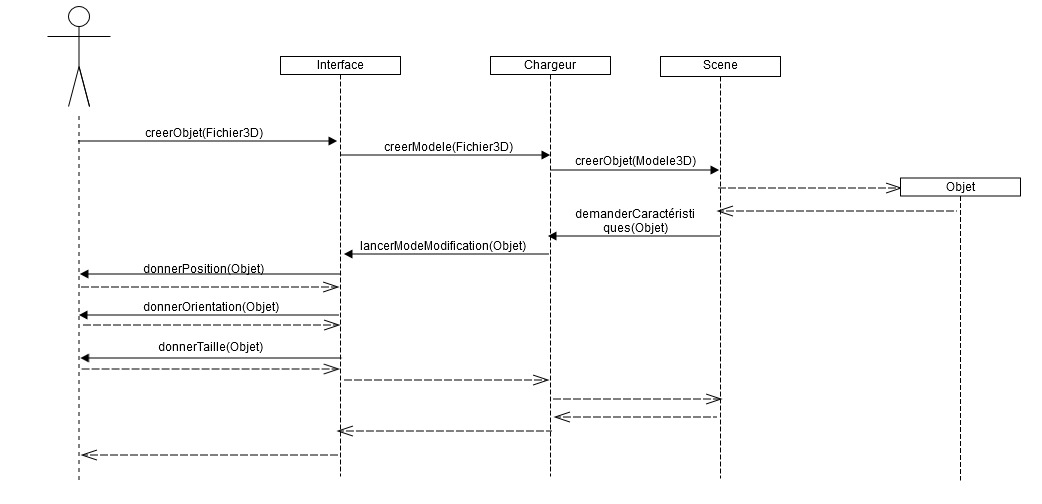
\includegraphics[scale=0.4]{creerobjet.jpg}
		\caption{\label{fig:creerObjet} Création d'un objet}
\end{figure}

\paragraph{}
Une fois la scène de travail créée, l'utilisateur pourra y ajouter des objets s'il le souhaite (cf. \ref{fig:creerObjet}). Pour cela, il va une fois de plus devoir communiquer avec l'interface graphique correspondante.

\paragraph{}
Une fois qu'il aura choisi un fichier objet d'extension .OBJ, .STL ou .PLY, l'interface enverra celui-ci au chargeur qui vérifiera sa validité et le transformera en un modèle 3D. Ce dernier sera transmis à la scène, qui se chargera de créer l'objet en plaçant les points du modèle par rapport à son origine. Enfin, une confirmation sera envoyée au chargeur, puis à l'interface, qui affichera la fenêtre correspondant au mode modification de l'objet.

\paragraph{}
Durant ce mode, l'interface demandera à l'utilisateur de modifier la position, l'orientation et la taille de l'objet s'il le souhaite, et appellera des méthodes soient publiques de l'objet, soit en passant par le chargeur puis la scène, pour effectuer les changements demandés.

\paragraph{}
Ce diagramme de séquence montre l'importance du chargeur dans l'intéraction de l'interface avec la scène. C'est lui qui s'occupera de créer la scène et de lui transmettre les demandes de l'utilisateur.


\newpage

\subsubsection{Déplacement dans la scène}

\begin{figure}[h]
		\centering
		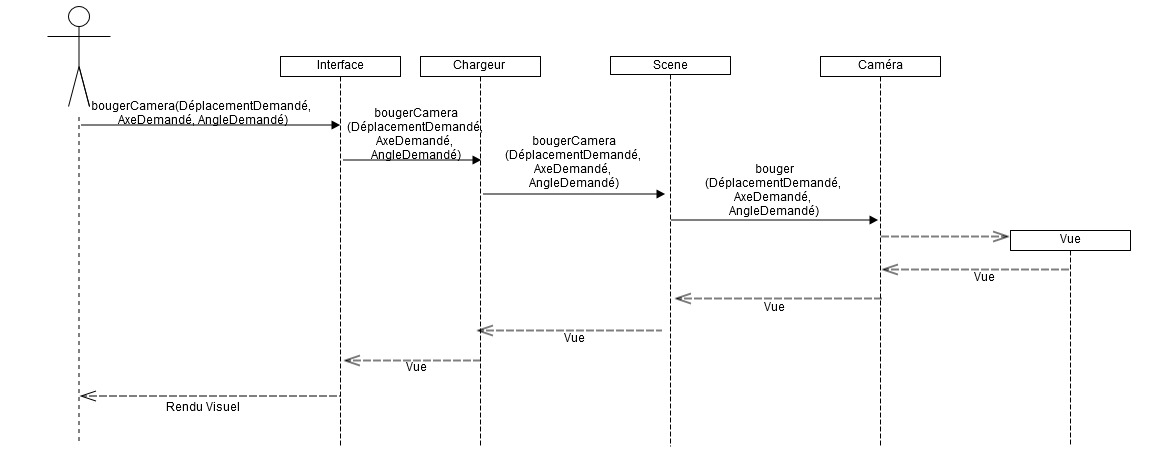
\includegraphics[scale=0.4]{bougerCamera.jpg}
		\caption{\label{fig:deplacementCam} Déplacement de la caméra}
\end{figure}

\paragraph{}
Quand il aura placé des objets dans sa scène, l’utilisateur pourra avoir envie de s’y déplacer pour observer les différents angles de vue (cf. \ref{fig:deplacementCam}). Pour cela, grâce à une action sur l’interface, il va demander à la caméra de se déplacer. La première demande sera donc initialisée par l’utilisateur, qui demandera le déplacement de la caméra à l’interface, selon un type (rotation, translation, homothétie), un axe (horizontal, vertical) et un angle ou une valeur donnée.

\paragraph{}
L’interface se chargera de transmettre l’information au chargeur, qui lui-même l’enverra à la caméra. Cette dernière se chargera de créer une nouvelle vue correspondant à la projection de la scène depuis l’angle demandé par l’utilisateur. Cette vue sera renvoyée étape par étape jusqu’à l’interface, qui se chargera de la transformer en un rendu visualisable par l’utilisateur dans la zone de la scène.

\subsubsection{Création d'un autostéréogramme}

\begin{figure}[h]
		\centering
		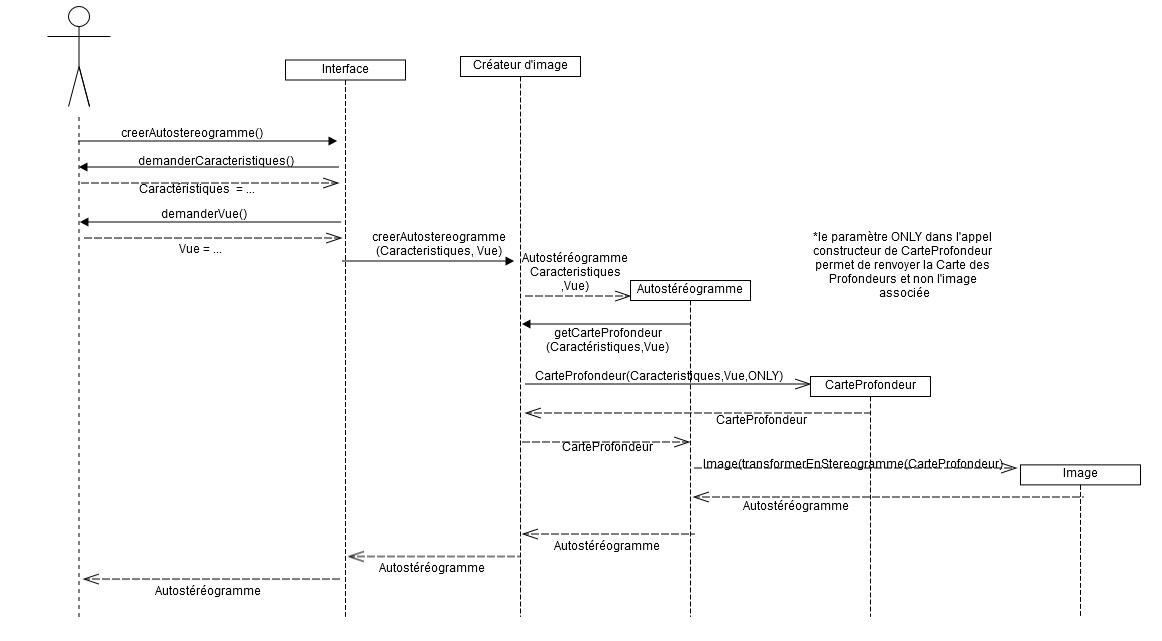
\includegraphics[scale=0.3]{creerstereogramme.jpg}
		\caption{\label{fig:creerAutostereogramme} Création d'un autostéréogramme}
\end{figure}

\paragraph{}
De la même façon que pour l’anaglyphe, c’est par l’intermédiaire de l’interface et du créateur d’image que l’utilisateur va créer son rendu (cf. \ref{fig:creerAutostereogramme}). Pour un autostéréogramme toutefois, un autre type de rendu sera également utilisé : la carte des profondeurs. C’est l’autostéréogramme qui demandera au créateur d’image de la créer pour lui, afin qu’il puisse l’utiliser pour générer l’autostéréogramme qu’il renverra vers l’utilisateur.

\newpage

\subsubsection{Création d'un flipbook}

\begin{figure}[h]
		\centering
		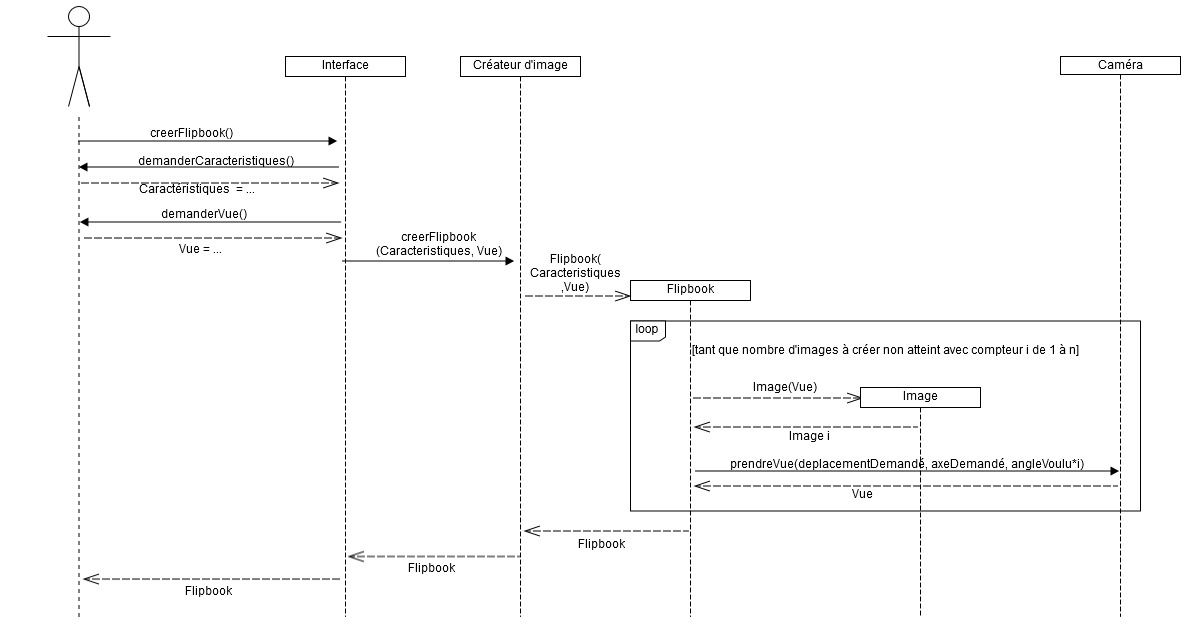
\includegraphics[scale=0.4]{creerflipbook.jpg}
		\caption{\label{fig:creerFlip} Création d'un flipbook}
\end{figure}

\paragraph{}
Une fois de plus, le passage entre l’utilisateur et le flipbook se fait par l’intermédiaire de l’interface et du créateur d’image (cf. \ref{fig:creerFlip}). Cette fois-ci toutefois, la génération se fera à l’aide d’une boucle qui permettra de remplir un vecteur d’image, qui sera renvoyé jusqu’à l’interface. Celle-ci se chargera de pouvoir afficher toutes les vues les unes après les autres dans la fenêtre d’affichage.

\newpage

\subsection{Diagrammes de classes}

\paragraph{}
A partir des diagrammes de séquences présentés précédemment, l’architecture du projet a pu être déterminée. La version finale de celle-ci dépendra grandement des bibliothèques OpenGL et Qt et des différentes utilisations de leurs modules.

\subsubsection{Diagramme de paquetages}

\begin{figure}[h]
		\centering
		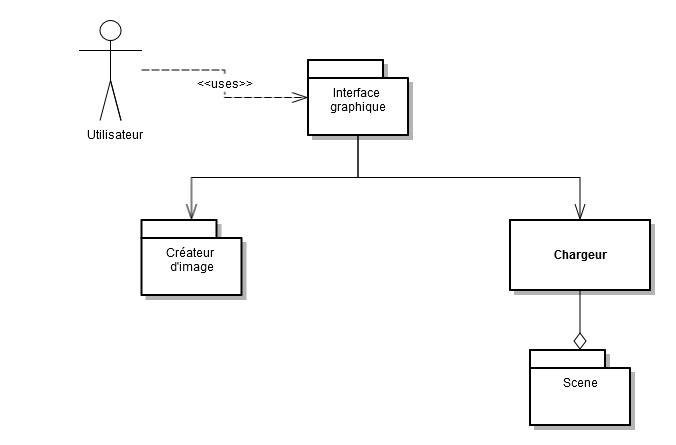
\includegraphics[scale=0.4]{diag_packages.jpg}
		\caption{\label{fig:diagPaquetage} Diagramme de paquetages}
\end{figure}

\paragraph{}
Ce premier diagramme représente l’architecture globale du futur logiciel (cf. \ref{fig:diagPaquetage}). Comme montré dans les diagrammes de séquence précédemment, le point d’entrée du logiciel pour l’utilisateur est l’interface graphique. C’est celle-ci qui redirigera les actions de l’utilisateur vers soit le créateur d’image, soit le chargeur. Ce dernier sera toujours utilisé pour accéder à la scène, car il sera responsable de la création de celle-ci et de la transformation des fichiers objets en modèles 3D.

\subsubsection{Paquetage Création}

\begin{figure}[h]
		\centering
		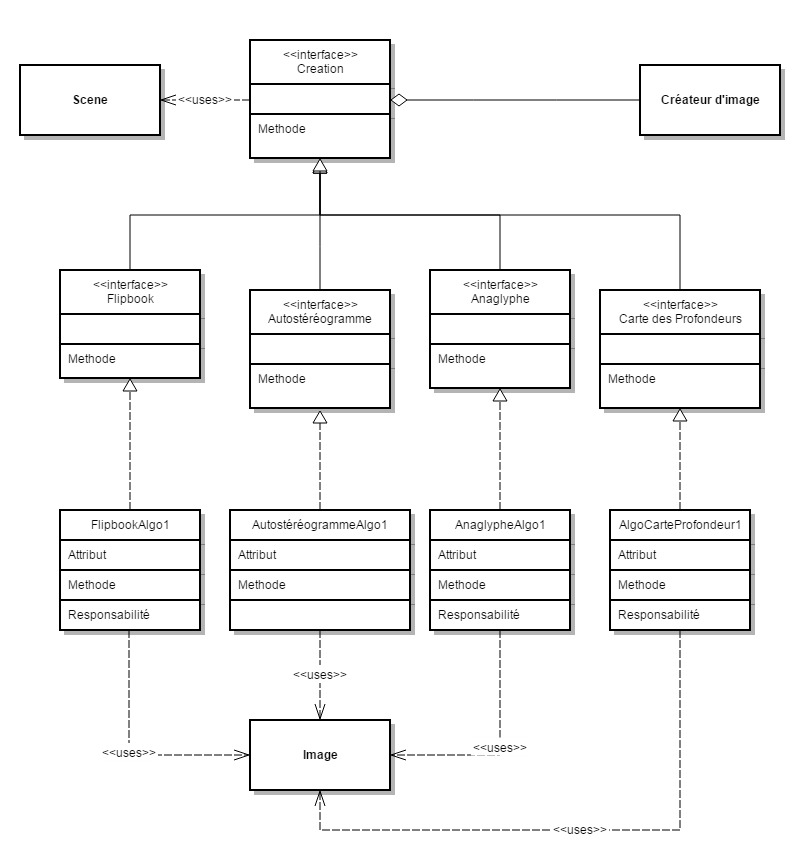
\includegraphics[scale=0.4]{package_creation.jpg}
		\caption{\label{fig:paqCreation} Architecture du paquetage Création}
\end{figure}

\paragraph{}
L’architecture du paquetage de création a été pensée pour que de futures extensions puissent être insérées à ce niveau du logiciel (cf. \ref{fig:paqCreation}). En effet, le créateur d’image génère un rendu, qui peut être l’un des types situés en dessous. Si l’on souhaite ajouter un nouveau rendu possible, il suffit donc de le placer au même niveau que les interfaces Flipbook, Autostéréogramme, etc. De la même façon, si l’on souhaite ajouter un algorithme différent pour obtenir l’un des rendus, il suffit de l’ajouter en-dessous de la classe virtuelle correspondante. Ainsi cette réalisation répond au besoin d’extensibilité.

\paragraph{}
Toutes les classes sont en relation avec la caméra par l’intermédiaire de la scène, de façon à pouvoir récupérer les différentes vues nécessaires à la création des rendus.

\newpage

\subsubsection{Paquetage Scène}

\begin{figure}[h]
		\centering
		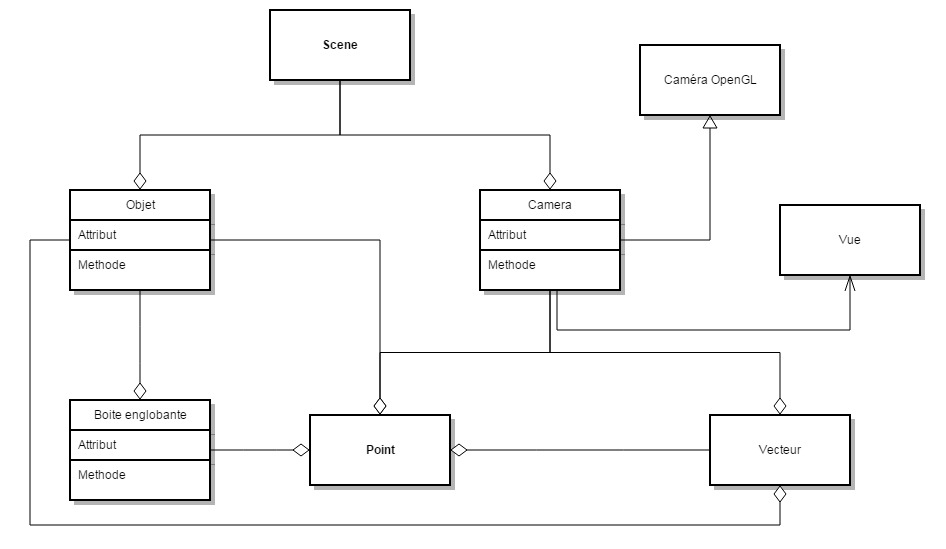
\includegraphics[scale=0.4]{package_scene.jpg}
		\caption{\label{fig:paqScene} Architecture du paquetage Scène}
\end{figure}

\paragraph{}
On considèrera pour le logiciel la scène comme un ensemble d’objets et une caméra. C’est la scène qui gèrera elle-même l’accès à ses différentes composantes (cf. \ref{fig:paqScene}). La caméra utilisée, qui sera liée à la caméra de la bibliothèque OpenGL, génèrera des vues qui pourront être utilisées pour l’affichage de la scène ou la création de rendus. Le contenu réel de ces vues et leur utilisation dépendront de la bibliothèque OpenGL.

\subsubsection{Paquetage Interface}

\begin{figure}[h]
		\centering
		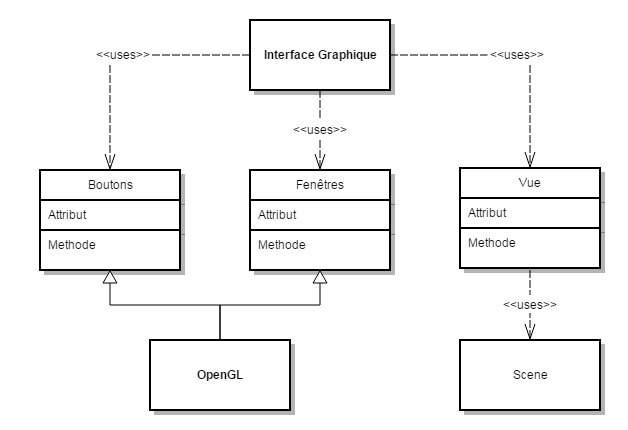
\includegraphics[scale=0.4]{package_interface.jpg}
		\caption{\label{fig:paqInterface} Architecture du paquetage Interface}
\end{figure}

\paragraph{}
Le paquetage Interface est le paquetage utilisé par l’utilisateur pour interagir avec le logiciel. L’interface sera constituée de boutons et de fenêtres, qui seront des produits de la bibliothèque Qt et du module OpenGL pour Qt (cf. \ref{fig:paqInterface}). L’affichage de la scène se fera à partir des vues générées par la Caméra de la Scène, comme expliqué dans la partie précédente.

\paragraph{}
La création de l’interface sera pensée pour que l’ajout de boutons et de fonctionnalités au logiciel se fasse de façon simple.

\newpage


\bibliographystyle{plain}
\bibliography{bibli}
%%% End document
\end{document}